\documentclass{article}

\usepackage[margin=1in]{geometry}
\usepackage{amsmath}
\usepackage{amssymb}
\usepackage{graphicx}
\usepackage{float}
\usepackage[section]{placeins}
\usepackage{parskip}
\usepackage{xcolor}
\usepackage{listings}
\usepackage[hidelinks]{hyperref}

% Figures are read from ../figures/ when this file is compiled inside report/.
% On Overleaf, upload the five PNGs next to this file or into a figures/ folder.
\graphicspath{{../figures/}{figures/}{./}}

\definecolor{codebg}{RGB}{245,245,245}
\definecolor{codegray}{RGB}{128,128,128}
\definecolor{codered}{RGB}{163,21,21}

\lstset{
  language=Python,
  basicstyle=\ttfamily\footnotesize,
  keywordstyle=\color{blue},
  stringstyle=\color{codered},
  commentstyle=\color{codegray}\itshape,
  backgroundcolor=\color{codebg},
  numbers=left,
  numberstyle=\tiny\color{codegray},
  frame=single,
  breaklines=true,
  showstringspaces=false,
  columns=fullflexible,
  keepspaces=true,
  captionpos=b
}

\title{Forecasting Lake Michigan--Huron Water Levels with Machine Learning:\\
A Comparison with a Water-Balance Model}
\author{Samundra Pathak\\ University of Wisconsin--Green Bay}
\date{October 19, 2026}

\begin{document}

\maketitle

\begin{abstract}
A machine learning model was built and evaluated to forecast the monthly mean water level of
Lake Michigan--Huron one to six months ahead, using 74 years of public data (1950--2023) from
the National Oceanic and Atmospheric Administration (NOAA) and the Great Lakes Observing System
(GLOS). The monthly over-lake precipitation, evaporation, river runoff and lake level were
merged into one table. A gradient boosting model was compared with persistence, a seasonal
climatology, a water-balance regression built on the physics of the lake, and a hybrid in which
the trees correct the errors of the water-balance model. Since this is time series data, a
rolling-origin backtest was used, in which each of the 44 test years (1980--2023) was forecast
by models trained only on the years before it. The water-balance model reached a root-mean-square
error (RMSE) of 3.22\,cm at one month and 14.66\,cm at six months. Gradient boosting was slightly
worse at every horizon (3.32\,cm and 15.39\,cm), but the differences were within the sampling
uncertainty, and the hybrid was no better than the water-balance model alone. When the
water-balance model was given the precipitation, evaporation and runoff that actually happened,
its error dropped to 2.39\,cm and 8.49\,cm. This result shows us that the limit on forecast
skill is the unknown future weather, not the flexibility of the model. In the final section, we
discuss the implications of these findings and suggest ways to improve the forecasts.
\end{abstract}

\section{Introduction}

The water level of the Great Lakes matters to a lot of people. Shoreline property owners,
shipping, harbors and wetlands all depend on it, and it can move a long way in only a few years.
Lake Michigan--Huron reached its lowest level on record in January 2013. Only seven and a half
years later, in July 2020, it was 1.88\,m higher and close to its record high. The rise in 2013
and 2014 alone was the fastest ever recorded on the lake over a two-year
period~\cite{gronewold2016}, and water levels across all of the Great Lakes kept rising for
several years after this period of record lows~\cite{gronewold2019}. Being able to forecast the
level a few months ahead is useful for anyone who has to plan around it.

Forecasting the lake level looks like a natural problem for machine learning, because long
public records exist for the level and for the water entering and leaving the lake. But unlike
a stock price, the lake level has well-understood physics behind it. The lake works like a
bathtub: the level changes only because water is added to it or removed from it. In this case
study, that fact is used as a test. A model built around the water balance of the lake is
compared with a flexible machine learning model that is given the same information and has to
find the structure by itself.

The lake that is used here is Lake Michigan--Huron. Lakes Michigan and Huron are joined at the
Straits of Mackinac and stand at the same elevation, so hydraulically they behave as one lake
with a surface area of about 117,400\,km$^2$~\cite{epa}. The goal of this case study is to build a complete
forecasting pipeline and to answer one narrow question: when forecasting the monthly mean level
one to six months ahead, does gradient boosting beat simple baselines, and does it beat a
physics-based water-balance model? The comparison is meant to be honest, including the case
where machine learning does not win.

\section{Data}

\subsection{Source}

All of the data used in this study is public. The monthly over-lake precipitation, over-lake
evaporation and river runoff for Lake Michigan and Lake Huron were retrieved from the Great Lakes
Monthly Hydrologic Data of the NOAA Great Lakes Environmental Research Laboratory
(GLERL)~\cite{glerl}, a database described by Hunter et al.~\cite{hunter2015}. The monthly
lake-wide mean water level was retrieved from the Seagull ERDDAP server of GLOS~\cite{glos}.
Levels are given in meters above the International Great Lakes Datum of 1985 (IGLD 1985), the
reference height used for all Great Lakes levels. In total, seven raw files were used
(Table~\ref{tab:data}), all of them downloaded on October 12, 2026. The raw files were never
modified; every change to the data was done in code.

\begin{table}[htbp]
\centering
\caption{The seven raw files used in this study.}
\label{tab:data}
\begin{tabular}{||l|c|c|c|c||}
\hline\hline
Variable & Source & Files & Units & Period with data \\
\hline\hline
Over-lake precipitation & NOAA GLERL & Michigan, Huron & mm per month & Jan 1940 -- Dec 2024 \\
Over-lake evaporation & NOAA GLERL & Michigan, Huron & mm per month & Jan 1940 -- Dec 2024 \\
Basin runoff & NOAA GLERL & Michigan, Huron & m$^3$/s & 1901 -- Aug 2024 \\
Lake level & GLOS & Michigan--Huron & m (IGLD 1985) & Jan 1918 -- Dec 2023 \\
\hline\hline
\end{tabular}
\end{table}

The download links for both sources are given in the references. The surface areas of the two
lakes were taken from the U.S.\ Environmental Protection Agency~\cite{epa}.

Two things were checked before the files were used. First, the level file is labeled
``Huron''. Since Michigan and Huron are one lake, it should be the level of the combined lake,
but that was worth checking. Its lowest value, 175.57\,m in January 2013, and its highest value,
177.50\,m in October 1986, are the known record low and record high of Lake Michigan--Huron, so
the series was used as the level of the combined lake. Second, Lake Michigan evaporation for
1941--1944 is almost the same from one year to the next, which real weather never is. These
years look filled in with modeled or average values, so the analysis starts in January 1950.
The level file runs to October 2025 but has no values after December 2023, so the analysis ends
there. Figure~\ref{fig:data} shows the level record and the average seasonal cycle of the
supply.

\begin{figure}[htbp]
\centering
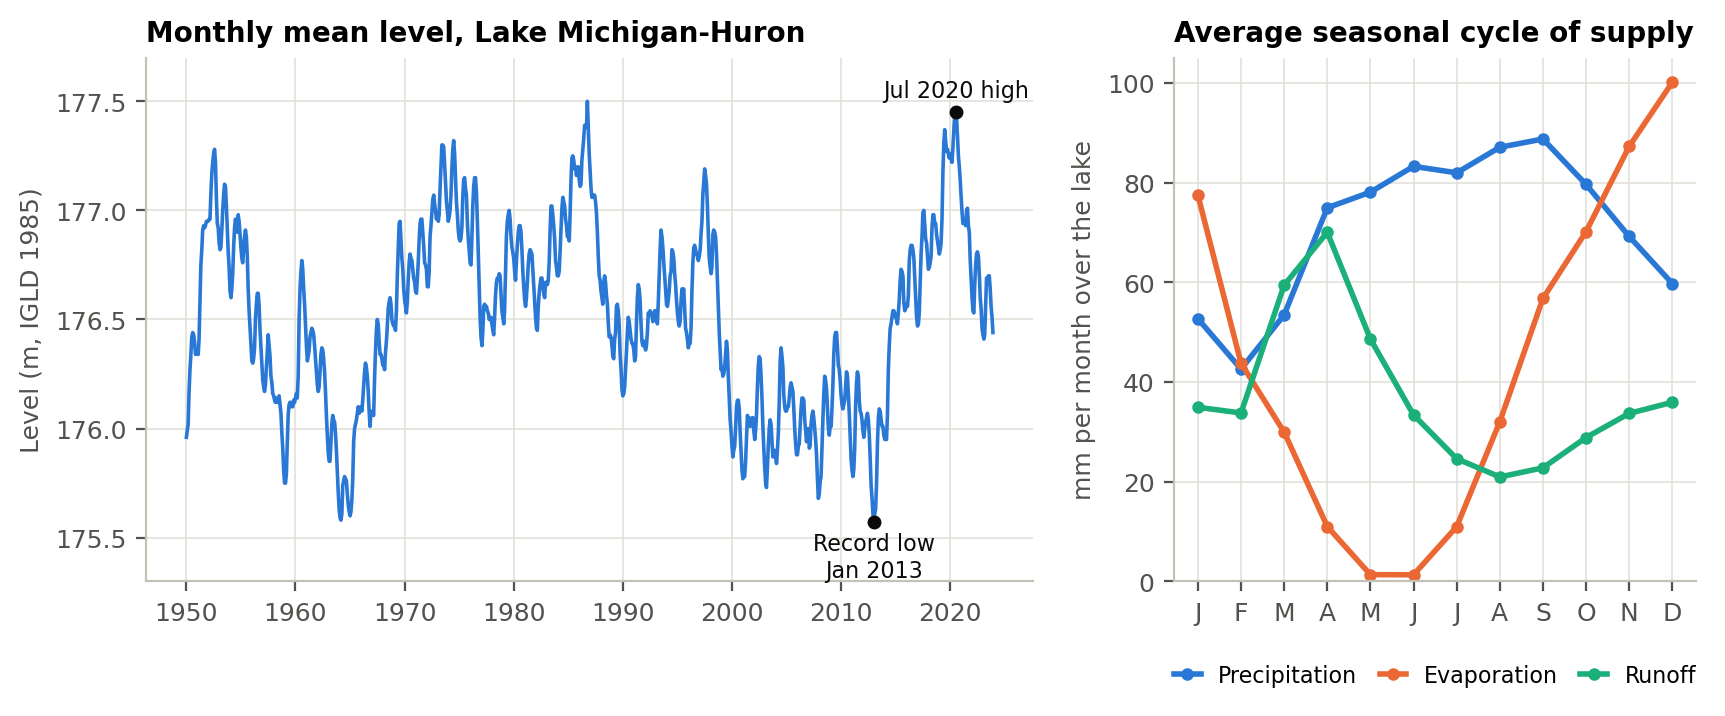
\includegraphics[width=\textwidth]{fig1_data_overview.png}
\caption{Left: monthly mean level of Lake Michigan--Huron, 1950--2023, with the January 2013
record low and the July 2020 high marked. Right: average seasonal cycle of precipitation,
evaporation and runoff over the lake. Runoff peaks with the spring snowmelt and evaporation peaks
in late autumn and early winter.}
\label{fig:data}
\end{figure}

\subsection{Building the Monthly Table}

The raw files come in different shapes and units. The precipitation and evaporation files have
one row per year with twelve monthly columns, while the runoff and level files have one row per
month. A few steps were needed to turn them into one table with one row per month:
\begin{itemize}
\item \textbf{Combining the Two Lakes}: Precipitation and evaporation are given as a depth of
water over each lake. Since Michigan and Huron are treated as one lake, the two depths were
combined as an area-weighted average,
\begin{align}
P_t &= w_M\,P^{\mathrm{Mic}}_t + w_H\,P^{\mathrm{Hur}}_t, \label{eq:precip}\\
w_M &= \frac{A_M}{A_M + A_H}, \qquad w_H = 1 - w_M, \label{eq:weights}
\end{align}
and the same was done for evaporation $E_t$. With $A_M = 57{,}800$\,km$^2$ and
$A_H = 59{,}600$\,km$^2$, the weights are $w_M = 0.492$ and $w_H = 0.508$.

\item \textbf{Runoff as a Depth}: Runoff is the river water draining from the land into the
lake. It is given as a flow in m$^3$/s for each basin, not as a depth. Flows add, so the two
basins were summed first. The total flow was then multiplied by the number of seconds in the
month to get a volume, and that volume was spread over the lake surface:
\begin{equation}
R_t = \frac{\left(Q^{\mathrm{Mic}}_t + Q^{\mathrm{Hur}}_t\right) \times N_t \times 86{,}400}
{A_M + A_H} \times 1000, \label{eq:runoff}
\end{equation}
where $N_t$ is the number of days in month $t$ and the areas are in m$^2$. As a check on the
scale, a typical combined runoff of 1,500\,m$^3$/s over a 30-day month is 33\,mm over the lake.
Because the lake is so large, one month of supply moves the level by only a few centimeters.

\item \textbf{Net Basin Supply (NBS)}: Now that all three terms are depths in mm, they can be
added. The result is the net basin supply, one of the standard hydrologic quantities for the
Great Lakes~\cite{glerl}:
\begin{equation}
\mathrm{NBS}_t = P_t - E_t + R_t. \label{eq:nbs}
\end{equation}
NBS is the amount the lake would rise in month $t$ if no water flowed in or out through the
rivers that connect it to the other lakes.

\item \textbf{Monthly Level Change}: The change in the monthly mean level from the previous
month, in mm:
\begin{equation}
\Delta L_t = 1000\left(L_t - L_{t-1}\right). \label{eq:dlevel}
\end{equation}

It can be noticed that the level record is a series of monthly means, not end-of-month values.
Suppose the level rises at a steady rate $s_t$ during month $t$, and let $\ell$ be the level at
the boundary between months $t-1$ and $t$. The mean level in month $t$ is then
$\ell + \tfrac{1}{2}s_t$, and the mean level in month $t-1$ is $\ell - \tfrac{1}{2}s_{t-1}$.
Subtracting the two gives
\begin{equation}
\Delta L_t = \tfrac{1}{2}\,s_{t-1} + \tfrac{1}{2}\,s_t. \label{eq:twomonth}
\end{equation}
This small fact is important to us because it shows that the change between two monthly means
depends equally on the supply of this month and of the month before. It is the reason the
water-balance model in Section~\ref{sec:wb} uses two months of every supply term.
\end{itemize}

Rows before 1950 and after the last month with every series present were then dropped. The
final table has 888 months, from January 1950 to December 2023, with no gaps and no missing
values. Table~\ref{tab:notation-data} summarizes the notation used in
Equations~\ref{eq:precip}--\ref{eq:twomonth}.

\begin{table}[htbp]
\centering
\caption{Notation used in building the monthly table.}
\label{tab:notation-data}
\begin{tabular}{||c|l||}
\hline\hline
Symbol & Meaning \\
\hline\hline
$t$ & Index of a month (a row in the table) \\
$L_t$ & Monthly mean lake level in month $t$ (m) \\
$\Delta L_t$ & Change in the monthly mean level from month $t-1$ to month $t$ (mm) \\
$P^{\mathrm{Mic}}_t,\ P^{\mathrm{Hur}}_t$ & Precipitation over Lake Michigan and over Lake Huron (mm) \\
$P_t,\ E_t,\ R_t$ & Precipitation, evaporation and runoff over the combined lake (mm) \\
$A_M,\ A_H$ & Surface areas of Lake Michigan and Lake Huron \\
$w_M,\ w_H$ & Area weights of the two lakes \\
$Q^{\mathrm{Mic}}_t,\ Q^{\mathrm{Hur}}_t$ & Runoff flowing into each lake (m$^3$/s) \\
$N_t$ & Number of days in month $t$ \\
$\mathrm{NBS}_t$ & Net basin supply, $P_t - E_t + R_t$ (mm) \\
$s_t$ & Rate at which the level rises during month $t$ \\
$\ell$ & Level at the boundary between months $t-1$ and $t$ \\
\hline\hline
\end{tabular}
\end{table}

Before building any model, a quick check was done to see whether the bathtub picture holds
(Figure~\ref{fig:wbcheck}). By Equation~\ref{eq:twomonth}, the monthly level change should
follow the mean NBS of this month and the previous month with a slope of 1. The fitted slope is
1.07 and the correlation is 0.81, so the picture holds well. The intercept is $-69$\,mm per
month. This is the water that leaves through the connecting rivers on average, which is not in
the dataset. Spread over the lake surface, it corresponds to a net outflow of roughly
3,100\,m$^3$/s.

\begin{figure}[htbp]
\centering
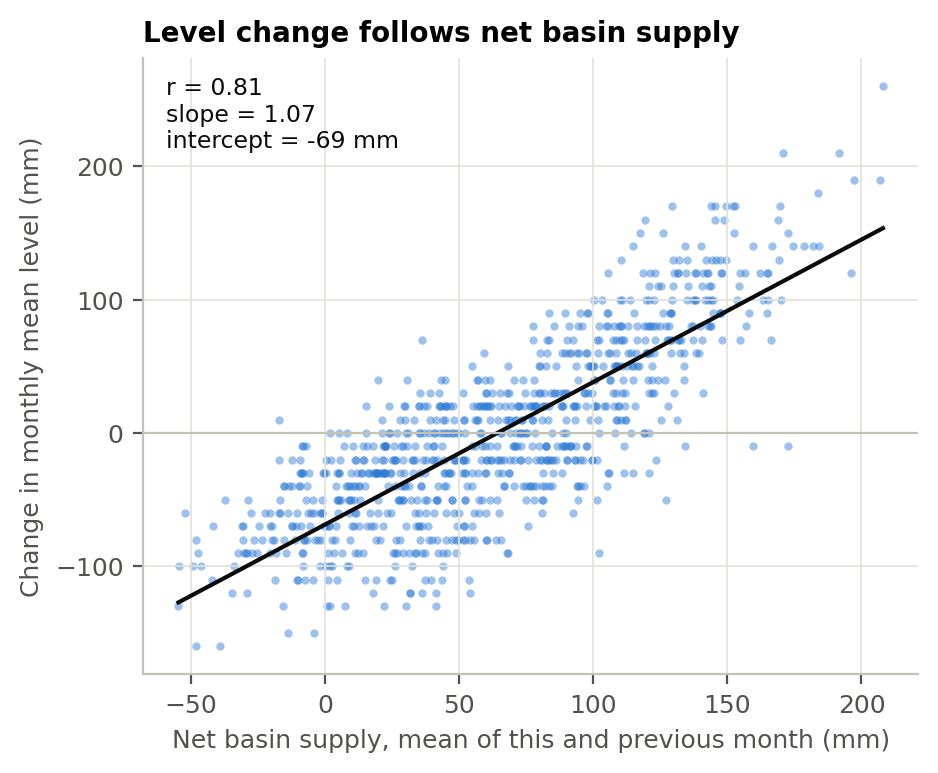
\includegraphics[width=0.55\textwidth]{fig2_water_balance_check.png}
\caption{Monthly level change against net basin supply (mean of this month and the previous
month), 1950--2023. The black line is a least-squares fit with a slope of 1.07 ($r = 0.81$).}
\label{fig:wbcheck}
\end{figure}

\subsection{Feature Engineering}

Feature engineering was only needed for the gradient boosting model, since the water-balance
model takes its inputs straight from the table. The idea was to give the gradient boosting model
the same information that the water-balance model sees, plus a longer memory. A total of 18
features were chosen, and every one of them is known at the end of month $t$:
\begin{itemize}
\item \textbf{Current Level}: The level relative to a reference level, $L_t - L_{\mathrm{ref}}$,
with $L_{\mathrm{ref}} = 176.5$\,m. The reference only centers the numbers and has no effect on
the forecasts.
\item \textbf{Recent Level Change}: The level change of the last three months, $\Delta L_t$,
$\Delta L_{t-1}$ and $\Delta L_{t-2}$.
\item \textbf{Precipitation, Evaporation and Runoff}: The values of $P$, $E$ and $R$ for the
last three months, nine features in total.
\item \textbf{Accumulated NBS}: The total supply over the last 3, 6 and 12 months,
\begin{equation}
S^{(w)}_t = \sum_{i=0}^{w-1} \mathrm{NBS}_{t-i}, \qquad w \in \{3, 6, 12\}. \label{eq:accum}
\end{equation}
\item \textbf{Season}: The calendar month $m$ of month $t$, written as two numbers,
\begin{equation}
\sin\!\left(\frac{2\pi m}{12}\right) \quad \text{and} \quad \cos\!\left(\frac{2\pi m}{12}\right).
\label{eq:season}
\end{equation}

It can be noticed that the month number by itself would be a poor feature, because it puts
December (12) and January (1) eleven steps apart even though they are neighbors. Placing the
months on a circle with a sine and a cosine fixes this: December and January end up next to each
other, just like any other pair of months in a row.
\end{itemize}

Rolling-window features need a warm-up period before they are defined (for example, the
12-month sum needs 12 months of history), so the first 11 months of 1950 were not used to train
this model. Table~\ref{tab:features} summarizes the features.

\begin{table}[htbp]
\centering
\caption{Features of the gradient boosting model at origin month $t$.}
\label{tab:features}
\begin{tabular}{||l|c|c||}
\hline\hline
Group & Features & Count \\
\hline\hline
Current level & $L_t - L_{\mathrm{ref}}$ & 1 \\
Recent level change & $\Delta L_t,\ \Delta L_{t-1},\ \Delta L_{t-2}$ & 3 \\
Precipitation & $P_t,\ P_{t-1},\ P_{t-2}$ & 3 \\
Evaporation & $E_t,\ E_{t-1},\ E_{t-2}$ & 3 \\
Runoff & $R_t,\ R_{t-1},\ R_{t-2}$ & 3 \\
Accumulated NBS & $S^{(3)}_t,\ S^{(6)}_t,\ S^{(12)}_t$ & 3 \\
Season & $\sin(2\pi m/12),\ \cos(2\pi m/12)$ & 2 \\
\hline\hline
Total & & 18 \\
\hline\hline
\end{tabular}
\end{table}

\subsection{Target Definition}

To calculate the target, a simple question was asked. Standing at the end of month $t$, how much
will the level change between now and $h$ months from now? The month $t$ is called the origin of
the forecast and $h$ is the horizon:
\begin{equation}
y_{t,h} = 1000\left(L_{t+h} - L_t\right), \qquad h = 1, 2, \dots, 6. \label{eq:target}
\end{equation}
The forecast level is then $\hat L_{t+h} = L_t + \hat y_{t,h}/1000$. A forecast is only allowed
to use the level and $P$, $E$, $R$ up to and including month $t$.

The models predict the change in level, not the level itself. The level this month is almost
identical to the level last month (their correlation is 0.987), so almost any model looks
impressive if its predicted levels are simply compared with the observed levels. The
month-to-month change is much harder to predict (its correlation with the previous month's
change is 0.703), and it is the part a forecast actually has to get right.

\subsection{Train/Test Split}

As we are dealing with time series data, a randomly selected train/test split would not work.
Neighboring months are strongly related and several features use rolling windows, so a random
split would leak information from the test period into the training period. A single
chronological split would avoid that, but it would test the models on only one stretch of years.

Instead, a rolling-origin backtest was used, which is also called evaluation on a rolling
forecasting origin~\cite{fpp3}. For each test year $Y$ from 1980 to 2023, every
model was trained again on all the months before January of year $Y$, and it then forecast every
month of $Y$ at every horizon. The forecast for target month $T$ at horizon $h$ is issued from
the origin $T - h$. After that, the training window grows by one year and the process repeats.
The first training set covers 1950--1979, so the first fit already has 30 years of data. This
gives $44 \times 12 = 528$ forecasts per model and horizon, and every model was fitted without
seeing any month of the year it was tested on.

\section{Methodology}

\subsection{Baseline Models}

Two simple models were built first. They are the benchmarks that any useful model has to beat.

\textbf{Persistence.} The simplest possible forecast is that the level stays where it is:
\begin{equation}
\hat y_{t,h} = 0. \label{eq:persistence}
\end{equation}

\textbf{Seasonal Climatology.} The lake rises every spring and falls every autumn
(Table~\ref{tab:clim}). On average it rises by about 29\,cm from March to July and falls by
about the same amount from August to February. This model forecasts that each future month will
change by the average change of that calendar month in the training years. If
$\overline{\Delta L}_m$ is the average of $\Delta L$ over all training months that fall in
calendar month $m$, and $m(t)$ is the calendar month of month $t$, then
\begin{equation}
\hat y_{t,h} = \sum_{k=1}^{h} \overline{\Delta L}_{m(t+k)}. \label{eq:climatology}
\end{equation}
Since the seasonal cycle is so regular, this is a difficult benchmark to beat. A model that only
learned the calendar would beat persistence easily, and that should not be mistaken for real
forecasting skill.

\begin{table}[htbp]
\centering
\caption{Average change in the monthly mean level for each calendar month, 1950--2023 (cm).}
\label{tab:clim}
\small
\begin{tabular}{||l|c|c|c|c|c|c|c|c|c|c|c|c||}
\hline\hline
Month & Jan & Feb & Mar & Apr & May & Jun & Jul & Aug & Sep & Oct & Nov & Dec \\
\hline\hline
Change & $-3.7$ & $-1.8$ & $+1.5$ & $+8.5$ & $+9.8$ & $+6.4$ & $+3.1$ & $-1.7$ & $-5.1$
& $-6.5$ & $-5.5$ & $-4.3$ \\
\hline\hline
\end{tabular}
\end{table}

\subsection{Water-Balance Model}
\label{sec:wb}

The water-balance model is built on the bathtub idea. The volume of water in the lake, $V$,
changes only through the water crossing its boundary:
\begin{equation}
\frac{dV}{dt} = A\,(p - e) + Q_R + Q_{\mathrm{in}} - Q_{\mathrm{out}}, \label{eq:volume}
\end{equation}
where $A$ is the lake surface area, $p$ and $e$ are the precipitation and evaporation rates over
the lake, $Q_R$ is the runoff from the land, $Q_{\mathrm{in}}$ is the inflow from Lake Superior
through the St.~Marys River, and $Q_{\mathrm{out}}$ is the outflow through the St.~Clair River.
The area barely changes over the observed range of levels, so $dV = A\,dL$, and dividing by $A$
turns every term into a depth of water:
\begin{equation}
\frac{dL}{dt} = p - e + \frac{Q_R}{A} + \frac{Q_{\mathrm{in}} - Q_{\mathrm{out}}}{A}.
\label{eq:bathtub}
\end{equation}
The first three terms are exactly the NBS of Equation~\ref{eq:nbs}. The two river flows are not
in the dataset, but their behavior is known in outline. The St.~Clair River is not regulated, so
its outflow grows when the lake is higher, roughly as
$Q_{\mathrm{out}} \approx Q_0 + k\,(L - L_{\mathrm{ref}})$ with $k > 0$. A high lake therefore
drains faster than a low one, and the level is always being pulled back toward an equilibrium.

This physics was turned into a linear regression:
\begin{equation}
\Delta L_t = a_{m(t)} + \sum_{c \in \{P,E,R\}} \left( b_{c,0}\,X_{c,t} + b_{c,1}\,X_{c,t-1}
\right) + g\left(L_{t-1} - L_{\mathrm{ref}}\right) + \varepsilon_t, \label{eq:wb}
\end{equation}
where $X_{P,t}$, $X_{E,t}$ and $X_{R,t}$ are $P_t$, $E_t$ and $R_t$. Every part of it has a
meaning:
\begin{itemize}
\item The two months of every supply term come from the monthly means
(Equation~\ref{eq:twomonth}).
\item The twelve monthly constants $a_m$ stand in for the average flow through the connecting
rivers, which changes through the year.
\item The level term $g\,(L_{t-1} - L_{\mathrm{ref}})$ is the outflow that grows with the level,
so $g$ should be negative.
\item For a perfect water budget, $b_{P,0} + b_{P,1} = 1$, $b_{E,0} + b_{E,1} = -1$ and
$b_{R,0} + b_{R,1} = 1$.
\end{itemize}
That is $12 + 6 + 1 = 19$ numbers to learn. They were found by ordinary least squares, which
picks the coefficients that make the sum of squared errors as small as possible:
\begin{equation}
F(\beta) = \sum_{t} \left( \Delta L_t - \widehat{\Delta L}_t \right)^2, \label{eq:ols}
\end{equation}
where $\beta$ collects all 19 coefficients and $\widehat{\Delta L}_t$ is the value of
Equation~\ref{eq:wb} without the error term $\varepsilon_t$.

\textbf{Forecasting with Unknown Weather.} To forecast, the future $P$, $E$ and $R$ are needed,
but they are unknown. Each one was replaced by its calendar-month average from the training
years, plus a fading share of how unusual the latest month was:
\begin{equation}
\hat X_{c,t+k} = \overline{X}_{c,m(t+k)} + \phi_c^{\,k}\left(X_{c,t} - \overline{X}_{c,m(t)}
\right), \label{eq:ar1}
\end{equation}
where $\phi_c$ is the correlation between one month's anomaly and the next month's anomaly in the
training data. This is called a first-order autoregression, or AR(1)~\cite{fpp3}. The model is then stepped
forward one month at a time, feeding its own predicted level back in:
\begin{equation}
\hat L_{t+k} = \hat L_{t+k-1} + \frac{\widehat{\Delta L}_{t+k}}{1000}, \qquad \hat L_t = L_t.
\label{eq:recursion}
\end{equation}

\textbf{Perfect Forcing.} The same model was also run with the observed future $P$, $E$ and $R$
in place of Equation~\ref{eq:ar1}. This uses information from the future, so it is not a real
forecast. It shows how good the model could be with a perfect weather forecast, which tells us
how much of the error comes from not knowing the weather.

Table~\ref{tab:notation-wb} summarizes the notation used in
Equations~\ref{eq:volume}--\ref{eq:recursion}.

\begin{table}[htbp]
\centering
\caption{Notation used in the water-balance model.}
\label{tab:notation-wb}
\begin{tabular}{||c|l||}
\hline\hline
Symbol & Meaning \\
\hline\hline
$V$ & Volume of water in the lake \\
$A$ & Surface area of the combined lake \\
$p,\ e$ & Precipitation and evaporation rates over the lake \\
$Q_R$ & Runoff from the land basin \\
$Q_{\mathrm{in}},\ Q_{\mathrm{out}}$ & Inflow from Lake Superior and outflow through the
St.~Clair River \\
$Q_0,\ k$ & Outflow at the reference level, and how fast the outflow grows with the level \\
$m(t)$ & Calendar month (1 to 12) of month $t$ \\
$X_{c,t}$ & Supply term $c$ (precipitation, evaporation or runoff) in month $t$ (mm) \\
$a_m$ & Constant for calendar month $m$ (mm) \\
$b_{c,0},\ b_{c,1}$ & Weights of supply term $c$ in this month and in the previous month \\
$g$ & Level coefficient (mm per month per meter of level) \\
$L_{\mathrm{ref}}$ & Reference level, 176.5\,m \\
$\varepsilon_t$ & Error term \\
$\beta$ & All 19 coefficients of the model \\
$\overline{X}_{c,m}$ & Average of supply term $c$ in calendar month $m$ over the training years \\
$\phi_c$ & Month-to-month correlation of the anomalies of supply term $c$ \\
$\hat X_{c,t+k},\ \hat L_{t+k}$ & Forecast supply and forecast level $k$ months after the origin \\
\hline\hline
\end{tabular}
\end{table}

\subsection{Gradient Boosting}

The machine learning model of choice here was gradient boosting~\cite{friedman2001} with
regression trees~\cite{cart}, from the scikit-learn library~\cite{sklearn}. A regression tree
splits the data with a series of yes-or-no questions
about the features (for example, \emph{was the runoff this month above 40\,mm?}) and predicts
the average target of each final group, called a leaf. One small tree is a weak model on its
own, but gradient boosting adds many of them together, and each new tree corrects the mistakes
left by the trees before it:
\begin{equation}
F_M(\mathbf{x}) = F_0 + \nu \sum_{j=1}^{M} T_j(\mathbf{x}), \label{eq:gb}
\end{equation}
where $F_0$ is the average of the training targets. Each tree $T_j$ is fitted to the residuals
of the model built so far,
\begin{equation}
r^{(j)}_i = y_i - F_{j-1}(\mathbf{x}_i), \label{eq:resid}
\end{equation}
which is the direction that reduces the squared error the fastest. The learning rate $\nu$
shrinks the step of each tree, so the model learns slowly and is less likely to overfit.

A separate model was trained for each horizon $h = 1, \dots, 6$, and each one predicts $y_{t,h}$
directly from the 18 features in Table~\ref{tab:features}. The settings were fixed in advance and
were not tuned on the test years (Table~\ref{tab:gbsettings}). Because each tree is fitted to a
random part of the training rows, this version is called stochastic gradient
boosting~\cite{friedman2002}.

\begin{table}[htbp]
\centering
\caption{Settings of the gradient boosting model.}
\label{tab:gbsettings}
\begin{tabular}{||l|c|l||}
\hline\hline
Setting & Value & Meaning \\
\hline\hline
Number of trees, $M$ & 300 & Trees added together in each model \\
Learning rate, $\nu$ & 0.03 & Shrinks the contribution of each tree \\
Maximum depth & 3 & Each tree asks at most three questions in a row \\
Subsample & 0.8 & Each tree is fitted to a random 80\% of the training rows \\
Minimum leaf size & 5 & Every leaf holds at least 5 months \\
Random seed & 0 & Makes the results repeatable \\
\hline\hline
\end{tabular}
\end{table}

\subsection{Hybrid Model}

The hybrid model combines the two approaches. The trees are not trained on the level change
itself, but on what the water-balance model got wrong:
\begin{equation}
\hat y^{\,\mathrm{hyb}}_{t,h} = \hat y^{\,\mathrm{WB}}_{t,h} + F^{(h)}_M(\mathbf{x}_t),
\qquad F^{(h)}_M \text{ trained on } y_{t,h} - \hat y^{\,\mathrm{WB}}_{t,h}. \label{eq:hybrid}
\end{equation}
This is the most direct test of whether machine learning can find a pattern that the
physics-based model misses. If the water-balance model leaves anything systematic behind, the
trees should find it.

Table~\ref{tab:notation-gb} summarizes the additional notation used in
Equations~\ref{eq:gb}--\ref{eq:hybrid}.

\begin{table}[htbp]
\centering
\caption{Additional notation used in the gradient boosting and hybrid models.}
\label{tab:notation-gb}
\renewcommand{\arraystretch}{1.3}
\begin{tabular}{||c|l||}
\hline\hline
Symbol & Meaning \\
\hline\hline
$\mathbf{x}_t$ & The 18 features at origin month $t$ \\
$y_i$ & Target of training row $i$ \\
$F_M$ & Gradient boosting model made of $M$ trees \\
$F_0$ & Average of the training targets \\
$T_j$ & The $j$-th regression tree \\
$\nu$ & Learning rate \\
$r^{(j)}_i$ & Residual of training row $i$ that tree $j$ is fitted to \\
$\hat y^{\,\mathrm{WB}}_{t,h}$ & Water-balance forecast of the level change \\
$\hat y^{\,\mathrm{hyb}}_{t,h}$ & Hybrid forecast of the level change \\
$F^{(h)}_M$ & Trees of the hybrid for horizon $h$, trained on the water-balance errors \\
\hline\hline
\end{tabular}
\end{table}

\subsection{Evaluation}

The accuracy of each model is reported as the root-mean-square error (RMSE) of the forecast
level, in cm, separately for each horizon:
\begin{equation}
\mathrm{RMSE}_h = \sqrt{\frac{1}{n} \sum_{i=1}^{n} \left(\hat L_{i,h} - L_i\right)^2},
\label{eq:rmse}
\end{equation}
where $L_i$ is the observed level in target month $i$, $\hat L_{i,h}$ is its forecast made $h$
months earlier, and the sum runs over the $n = 528$ target months. The improvement of a model
over a reference model is the relative reduction in RMSE,
\begin{equation}
\mathrm{Skill}_h = 1 - \frac{\mathrm{RMSE}^{\,\mathrm{model}}_h}{\mathrm{RMSE}^{\,\mathrm{ref}}_h}.
\label{eq:skill}
\end{equation}

A small difference in RMSE between two models could just be luck. To check whether a difference
is real, the 44 test years were resampled with replacement 2,000 times, which is called a
bootstrap~\cite{efron1994}. For each resample, the RMSE difference between the two models was
computed again, and the middle 95\% of the 2,000 differences gives a 95\% interval. Whole years
were resampled together, because the errors within a year, and across overlapping multi-month
forecasts, are strongly related to each other. Resampling whole blocks of neighboring
observations instead of single values is known as a block bootstrap~\cite{kunsch1989}.

To see which inputs the gradient boosting model actually uses, its permutation importance was
measured~\cite{breiman2001}. For this, the model was trained on 1950--2009 and scored on 2010--2023. One group of
features $G$ was shuffled at a time, which destroys the information in that group while keeping
its values realistic, and the increase in RMSE was recorded:
\begin{equation}
I_G = \frac{1}{20} \sum_{q=1}^{20} \mathrm{RMSE}_q\left(G \text{ shuffled}\right)
- \mathrm{RMSE}\left(\text{nothing shuffled}\right). \label{eq:perm}
\end{equation}
Table~\ref{tab:metrics} explains each of these metrics.

\begin{table}[htbp]
\centering
\caption{Explanation of the metrics used to evaluate the models.}
\label{tab:metrics}
\begin{tabular}{||l|p{0.62\textwidth}||}
\hline\hline
Metric & Description \\
\hline\hline
RMSE & The typical size of a forecast miss, in cm. Errors are squared before they are averaged,
so large misses count more than small ones. Lower is better. \\
Skill & The fraction by which a model reduces the RMSE of a reference model. 0\% means no
improvement and 100\% means a perfect forecast. \\
95\% interval & The range that holds the middle 95\% of the 2,000 bootstrap differences between
two models. If it includes zero, the two models cannot be told apart. \\
Permutation importance & How much the RMSE increases when one group of features is shuffled. The
larger the increase, the more the model depends on that group. \\
\hline\hline
\end{tabular}
\end{table}

\section{Results}

\subsection{Accuracy by Horizon}

Table~\ref{tab:rmse} and Figure~\ref{fig:rmse} show the RMSE of every model at every horizon.

\begin{table}[htbp]
\centering
\caption{RMSE of the forecast level (cm) by horizon $h$ in months, test years 1980--2023. Bold
marks the best real forecast at each horizon. The last row uses the observed future weather and
is not a real forecast.}
\label{tab:rmse}
\begin{tabular}{||l|c|c|c|c|c|c||}
\hline\hline
Model & $h=1$ & $h=2$ & $h=3$ & $h=4$ & $h=5$ & $h=6$ \\
\hline\hline
Persistence & 6.73 & 12.37 & 17.06 & 20.73 & 23.30 & 24.81 \\
Seasonal climatology & 4.14 & 7.06 & 9.48 & 11.63 & 13.53 & 15.27 \\
Water balance & \textbf{3.22} & \textbf{6.33} & \textbf{8.82} & \textbf{11.03} & \textbf{12.96}
& 14.66 \\
Gradient boosting & 3.32 & 6.52 & 9.13 & 11.42 & 13.51 & 15.39 \\
Hybrid (water balance + boosting) & 3.27 & 6.36 & 8.97 & 11.18 & 12.98 & \textbf{14.59} \\
\hline\hline
Water balance, perfect forcing & 2.39 & 3.77 & 5.08 & 6.29 & 7.43 & 8.49 \\
\hline\hline
\end{tabular}
\end{table}

\begin{figure}[htbp]
\centering
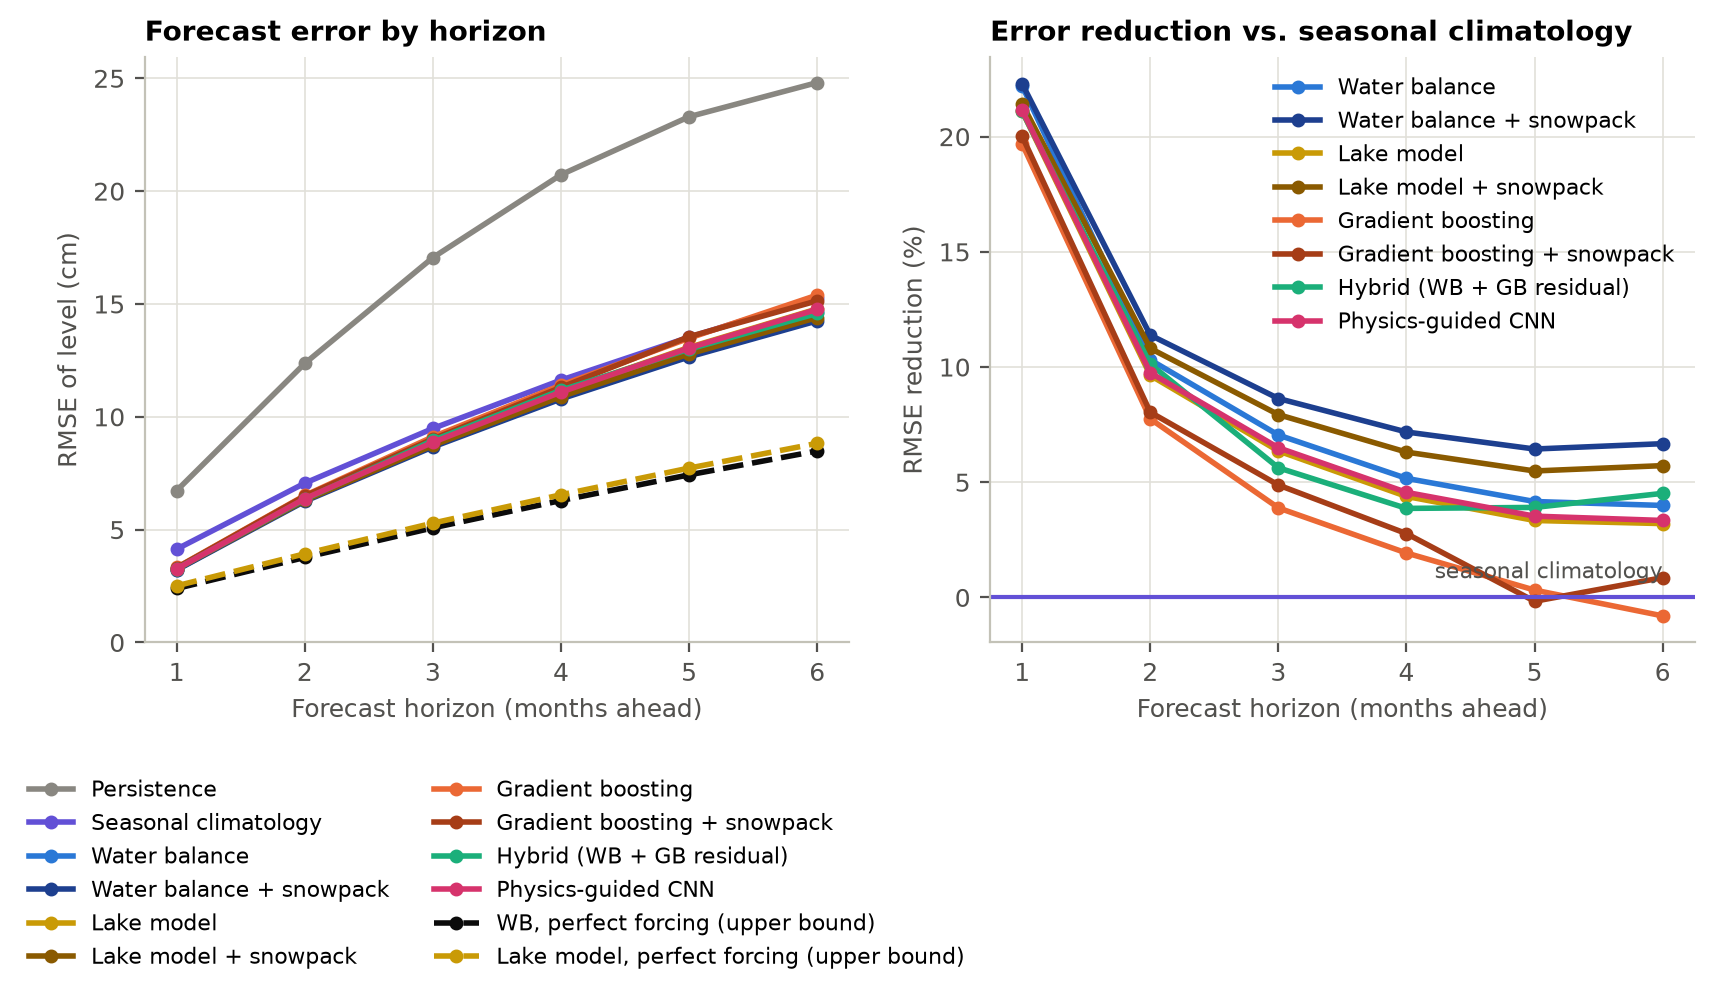
\includegraphics[width=\textwidth]{fig3_rmse_by_horizon.png}
\caption{Left: RMSE of the forecast level by horizon for every model. Right: reduction in RMSE
relative to the seasonal climatology.}
\label{fig:rmse}
\end{figure}

The main results are:
\begin{itemize}
\item \textbf{Every Model Beats Persistence}: The water-balance model reduces the RMSE of
persistence by 52\% at one month and 41\% at six months. But the seasonal climatology alone
already reduces it by 38--44\%, so most of that improvement comes from simply knowing the time of
year.
\item \textbf{Skill Beyond the Season Fades Quickly}: Compared with the seasonal climatology,
the water-balance model reduces the RMSE by 22\% at one month, 10\% at two months, 7\% at three
months and only 4--5\% at four to six months.
\item \textbf{Gradient Boosting Did Not Win}: It had a slightly higher RMSE than the
water-balance model at every horizon, and at five and six months it was no better than the
seasonal climatology.
\item \textbf{The Hybrid Did Not Help}: Letting the trees correct the water-balance errors
changed the RMSE by only $-0.08$ to $+0.15$\,cm.
\item \textbf{The Weather Sets the Limit}: With the observed future weather, the same
water-balance model reached 2.39\,cm at one month and 8.49\,cm at six months. That is 26\% lower
than the real water-balance forecast at one month and 40--43\% lower at two to six months. The
gap between this line and the real forecasts in Figure~\ref{fig:rmse} is far larger than any gap
between the models.
\end{itemize}

\subsection{Is the Difference Real?}

Table~\ref{tab:boot} shows the bootstrap comparison for the four most important pairs of models.

\begin{table}[htbp]
\centering
\caption{Difference in RMSE (cm) between two models, with the 95\% bootstrap interval in
brackets. GB is gradient boosting and WB is the water-balance model. A negative value means the
first model is better.}
\label{tab:boot}
\small
\begin{tabular}{||c|c|c|c|c||}
\hline\hline
Horizon & GB $-$ WB & Hybrid $-$ WB & WB $-$ Climatology & GB $-$ Climatology \\
\hline\hline
1 & $+0.10$\ \ $[-0.02,\ 0.23]$ & $+0.05$\ \ $[-0.03,\ 0.13]$ & $-0.92$\ \ $[-1.12,\ -0.70]$
& $-0.81$\ \ $[-1.04,\ -0.58]$ \\
2 & $+0.19$\ \ $[-0.06,\ 0.45]$ & $+0.03$\ \ $[-0.15,\ 0.20]$ & $-0.73$\ \ $[-1.17,\ -0.28]$
& $-0.54$\ \ $[-0.96,\ -0.13]$ \\
3 & $+0.32$\ \ $[-0.07,\ 0.70]$ & $+0.15$\ \ $[-0.16,\ 0.47]$ & $-0.67$\ \ $[-1.26,\ -0.08]$
& $-0.35$\ \ $[-0.94,\ 0.22]$ \\
4 & $+0.39$\ \ $[-0.13,\ 0.93]$ & $+0.15$\ \ $[-0.31,\ 0.63]$ & $-0.60$\ \ $[-1.41,\ 0.20]$
& $-0.21$\ \ $[-0.95,\ 0.49]$ \\
5 & $+0.54$\ \ $[-0.14,\ 1.23]$ & $+0.02$\ \ $[-0.55,\ 0.61]$ & $-0.56$\ \ $[-1.59,\ 0.48]$
& $-0.02$\ \ $[-0.85,\ 0.83]$ \\
6 & $+0.72$\ \ $[-0.16,\ 1.62]$ & $-0.08$\ \ $[-0.77,\ 0.65]$ & $-0.61$\ \ $[-1.99,\ 0.65]$
& $+0.11$\ \ $[-1.01,\ 1.20]$ \\
\hline\hline
\end{tabular}
\end{table}

The gap between gradient boosting and the water-balance model grows from 0.10\,cm at one month to
0.72\,cm at six months, but every one of its intervals includes zero. So gradient boosting is no
better than the water-balance model, and possibly slightly worse. Every interval for the hybrid
also includes zero. The water-balance model is clearly better than the seasonal climatology at
one to three months, where the whole interval is below zero, but not at four to six months.
Gradient boosting is clearly better than the seasonal climatology only at one and two months.

\subsection{What the Water-Balance Model Learned}

Table~\ref{tab:coef} lists the coefficients of Equation~\ref{eq:wb} fitted on the full record.

\begin{table}[htbp]
\centering
\caption{Water-balance weights of the supply terms fitted on 1950--2023, and the
month-to-month correlation $\phi_c$ of each supply term. The weights have no units (mm of level
change per mm of supply).}
\label{tab:coef}
\begin{tabular}{||l|c|c|c|c|c||}
\hline\hline
Supply term & $b_{c,0}$ & $b_{c,1}$ & Sum & Expected & $\phi_c$ \\
\hline\hline
Precipitation & $0.35$ & $0.53$ & $0.88$ & $+1$ & $0.02$ \\
Evaporation & $-0.43$ & $-0.37$ & $-0.81$ & $-1$ & $0.26$ \\
Runoff & $1.22$ & $0.61$ & $1.83$ & $+1$ & $0.45$ \\
\hline\hline
\end{tabular}
\end{table}

The coefficients make physical sense in sign. Both months of every supply term carry weight, just
as Equation~\ref{eq:twomonth} predicts. The sums for precipitation (0.88) and evaporation
($-0.81$) are reasonably close to the $\pm 1$ expected from the water budget. The twelve monthly
constants $a_m$ are all negative, from $-136$\,mm per month in October to $-67$\,mm per month in
May, which mostly reflects the net loss of water through the connecting rivers.

The level coefficient is $g = -23$\,mm per month per meter of level. It is negative, which
matches an outflow that grows as the lake rises. Its size means that an unusually high or low
level fades with a time scale of
\begin{equation}
\tau = \frac{1000\ \text{mm per meter}}{23\ \text{mm per month per meter}} \approx 43\
\text{months} \approx 3.6\ \text{years}. \label{eq:tau}
\end{equation}
This is a value implied by the regression, not a measurement of the river. It does show why the
lake has a memory of several years: an anomaly in the level fades over years, not months.

The runoff weights sum to 1.83. Runoff should not raise the lake by more than its own volume, so
runoff must be standing in for something that is not measured. Two likely candidates are the
inflow from Lake Superior, which tends to be high in the same wet periods, and runoff from parts
of the basin without river gauges. The model should therefore be read as shaped by physics, not
as a closed water budget.

The supply terms are barely predictable from their own past: $\phi_c$ is 0.02 for
precipitation, 0.26 for evaporation and 0.45 for runoff. In Equation~\ref{eq:ar1} the anomaly is
multiplied by $\phi_c^{\,k}$, so even for runoff only $0.45^3 \approx 9\%$ of an anomaly is left
after three months. This is why the skill fades so quickly: after a month or two, the best guess
for the future supply is just the seasonal average.

\subsection{What the Machine Learning Model Relies On}

\begin{figure}[htbp]
\centering
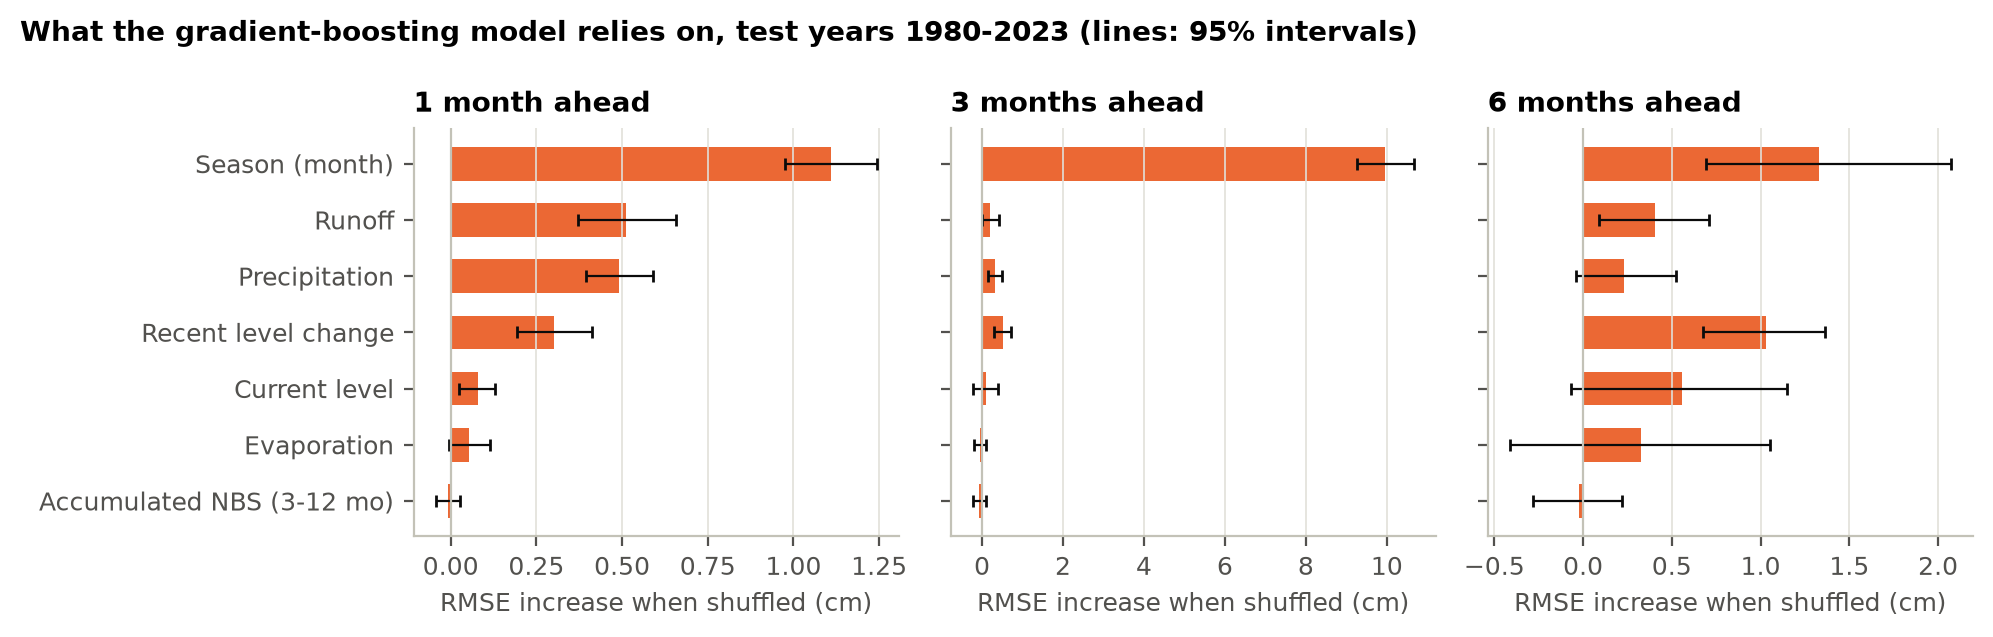
\includegraphics[width=\textwidth]{fig4_feature_importance.png}
\caption{Permutation importance for the gradient boosting model, trained on 1950--2009 and scored
on 2010--2023. Each bar shows how much the RMSE increases when one group of features is
shuffled.}
\label{fig:importance}
\end{figure}

At one month ahead, the model relies on recent runoff, the season, evaporation, the latest level
change and precipitation, in that order (Figure~\ref{fig:importance}). This matches the physics:
by Equation~\ref{eq:twomonth}, last month's supply is still working its way into this month's
mean level. At three months the model is dominated by the season. At six months the largest
group is evaporation and not the season, but evaporation has such a strong seasonal cycle
(Figure~\ref{fig:data}) that the model is most likely using it as another way of reading the
time of year. Permutation importance cannot separate features that carry the same information,
so the order among the seasonal features should not be over-interpreted. The clear finding is
that at longer horizons the model has learned the seasonal cycle and little else.

\subsection{Case Study: The 2013 Low to the 2020 High}

\begin{figure}[H]
\centering
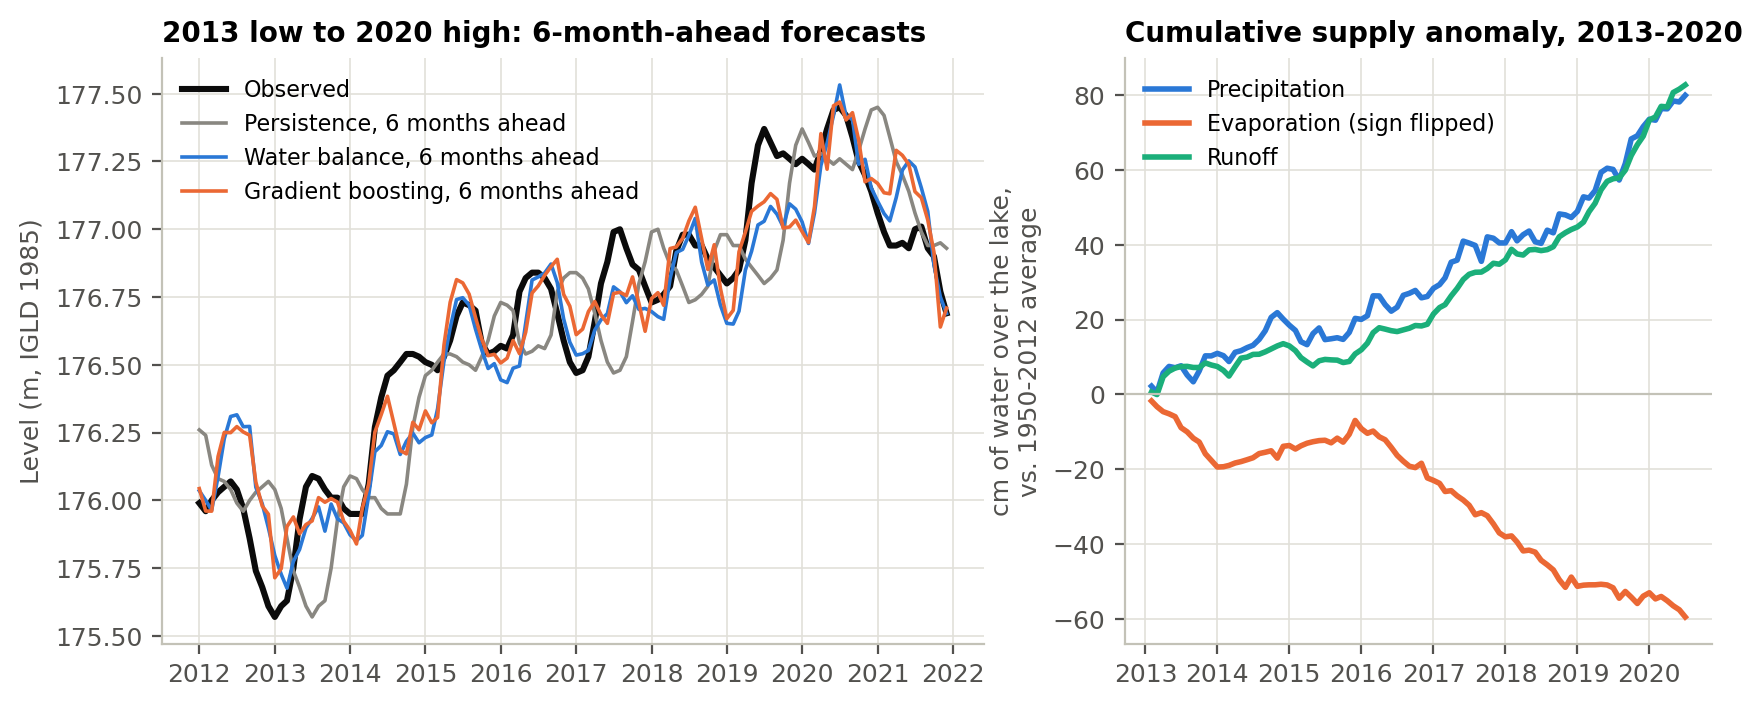
\includegraphics[width=\textwidth]{fig5_case_study_2013_2020.png}
\caption{Left: observed level and six-month-ahead forecasts, 2012--2021. Right: cumulative
anomalies of the supply terms from February 2013 to July 2020, relative to the 1950--2012
monthly averages. Evaporation is plotted with its sign flipped, so that upward always means more
water in the lake.}
\label{fig:case}
\end{figure}

Between January 2013 and July 2020 the lake rose 1.88\,m. Compared with the 1950--2012 averages,
the precipitation over the lake delivered about 80\,cm of extra water during this period and the
runoff about 83\,cm (Figure~\ref{fig:case}, right). Evaporation was below average in 2014 and
2015, which Gronewold et al.~\cite{gronewold2016} also found for 2014, but over the whole period
it worked in the opposite direction: it was above average and removed about 59\,cm more water
than usual. So the rise was driven by a long wet period, not by lower evaporation, which agrees
with the high precipitation and river flows reported for these
years~\cite{gronewold2016,gronewold2019}. The net supply anomaly, about $+1.0$\,m, is smaller
than the observed rise, and the rest cannot be explained with this dataset. Likely contributors
are the normal seasonal rise from January to July (about 27\,cm on average), lower outflow while
the lake was low, and the inflow from Lake Superior, which was very high in
2014~\cite{gronewold2016}.

Both the water-balance model and gradient boosting followed the rise at a six-month lead with
similar accuracy, with an RMSE of 15.0 and 14.6\,cm for target months in 2013--2020, against
26.7\,cm for persistence. Neither one saw it coming. Figure~\ref{fig:case} shows both of them
lagging behind the two steepest climbs, in 2014 and 2019. This is exactly what is expected from a
model that fills in the future supply with averages: it can follow a rise step by step as the wet
months arrive, but it cannot know in advance that the next six months will be wet again.

\section{Discussion}

The results of this case study point to one main finding: the two approaches reach almost the
same accuracy, and the simpler one is never worse. The reason can be seen in the physics.
Equation~\ref{eq:bathtub} is linear in the supply terms, so a linear regression with the right
inputs already has the correct shape. The trees have to rediscover that shape from only a few
hundred training months, and they have nothing to gain from being non-linear. The hybrid model
shows the same thing from the other side: when the trees were asked only for what the
water-balance model missed, they found nothing systematic.

The perfect-forcing run shows where the real limit is. Knowing the future weather would cut the
six-month error of the water-balance model from 14.66\,cm to 8.49\,cm, a 42\% reduction, which is
far more than any change of model achieved. Precipitation has almost no memory from one month to
the next ($\phi_P = 0.02$), so no model that only looks at past data can know whether the coming
months will be wet.

This study also has some limitations:
\begin{enumerate}
\item \textbf{Level Data End in 2023}: The level file runs to October 2025 but has no values after
December 2023, so 2024 could not be tested.
\item \textbf{Early Evaporation Data}: Lake Michigan evaporation for 1941--1944 appears to be
filled in, so the analysis starts in 1950.
\item \textbf{Changing Runoff Coverage}: The share of each basin with river gauges changes over
time (Michigan 0.78--0.98, Huron 0.74--0.93 during 1950--2023). It is kept in the table as a
data-quality column but is not used as a feature. Coverage drops sharply in 2024, when Huron is
only about 60\% gauged, and runoff is missing after August 2024. This is outside the analysis
period, but it matters for any extension.
\item \textbf{No Connecting-River Flows}: The St.~Marys inflow, the St.~Clair outflow and the
Chicago diversion are not in the dataset. The model represents them only through the monthly
constants and the level term, and the inflated runoff weight suggests that other terms are
absorbing part of this gap.
\item \textbf{Slow Drift}: Evaporation averaged 37--40\,mm per month in the 1970s--1990s and
51--52\,mm per month since 2010. On average the forecasts are slightly too high, by about
1--2\,cm at six months for the real forecasts and 4.8\,cm for the perfect-forcing run. This is a
sign of slow changes that a model trained on earlier decades does not fully capture.
\item \textbf{Level Resolution}: Levels are reported to the nearest centimeter, which adds a
small amount of rounding noise to the monthly changes.
\item \textbf{One Machine Learning Model}: Only one algorithm with one fixed setting was tested,
on a few hundred training months. The result shows that a reasonable off-the-shelf model does
not beat the water-balance model here. It does not show that no machine learning approach could.
\item \textbf{Data Delay}: $P$, $E$ and $R$ for month $t$ are assumed to be known at the end of
month $t$. In practice these estimates are published later, so the real-time skill would be
somewhat lower.
\end{enumerate}

\section{Conclusion}

This case study built a complete forecasting pipeline for the monthly level of Lake
Michigan--Huron and compared a machine learning model with a model built on the physics of the
lake. A 19-parameter water-balance regression was at least as accurate as gradient boosting at
every horizon from one to six months, and a hybrid of the two was no better than the
water-balance model alone. Most of the improvement over persistence came from the seasonal
cycle. Knowing the recent supply added a further 22\% at one month and little beyond three
months. The run with the observed weather showed that the error could be cut by more than 40\%
at two to six months if the future precipitation, evaporation and runoff were known.

The practical lesson is that the next improvement is more likely to come from better inputs than
from a more flexible model. Useful inputs would be seasonal climate forecasts of precipitation
and temperature, the snowpack at the end of winter (which controls the spring runoff), the lake
surface temperature and ice cover (which control evaporation), and measured flows in the
connecting rivers. Machine learning may well earn its place once those inputs are available, and
this backtest gives the baseline to test it against.

\begin{thebibliography}{99}
\raggedright

\bibitem{gronewold2016}
A.~D. Gronewold, J.~Bruxer, D.~Durnford, et al. Hydrological drivers of record-setting water
level rise on Earth's largest lake system. \emph{Water Resources Research}, 52(5):4026--4042,
2016. \url{https://doi.org/10.1002/2015WR018209}

\bibitem{gronewold2019}
A.~D. Gronewold and R.~B. Rood. Recent water level changes across Earth's largest lake system
and implications for future variability. \emph{Journal of Great Lakes Research}, 45(1):1--3,
2019. \url{https://doi.org/10.1016/j.jglr.2018.10.012}

\bibitem{epa}
U.S.\ Environmental Protection Agency. Physical features of the Great Lakes.
\url{https://www.epa.gov/greatlakes/physical-features-great-lakes} (accessed October 19, 2026).

\bibitem{glerl}
NOAA Great Lakes Environmental Research Laboratory. Great Lakes monthly hydrologic data
(1860--2024). \url{https://www.glerl.noaa.gov/ahps/mnth-hydro.html}. Data files:
\url{https://www.glerl.noaa.gov/pubs/tech_reports/glerl-083/UpdatedFiles/} (downloaded October
12, 2026).

\bibitem{hunter2015}
T.~S. Hunter, A.~H. Clites, K.~B. Campbell and A.~D. Gronewold. Development and application of
a North American Great Lakes hydrometeorological database, Part I: Precipitation, evaporation,
runoff, and air temperature. \emph{Journal of Great Lakes Research}, 41(1):65--77, 2015.
\url{https://doi.org/10.1016/j.jglr.2014.12.006}

\bibitem{glos}
GLISA, the NOAA Great Lakes CAP/RISA Team. Huron - Monthly - GLISA - General (dataset
\texttt{glisa\_general\_monthly\_huron}). Great Lakes Observing System, Seagull ERDDAP server.
\url{https://seagull-erddap.glos.org/erddap/info/glisa_general_monthly_huron/index.html}. Data
file: \url{https://seagull-erddap.glos.org/erddap/tabledap/glisa_general_monthly_huron.csv}
(downloaded October 12, 2026).

\bibitem{fpp3}
R.~J. Hyndman and G.~Athanasopoulos. \emph{Forecasting: Principles and Practice}, 3rd edition.
OTexts, Melbourne, Australia, 2021. \url{https://otexts.com/fpp3/}

\bibitem{friedman2001}
J.~H. Friedman. Greedy function approximation: A gradient boosting machine. \emph{The Annals of
Statistics}, 29(5):1189--1232, 2001. \url{https://doi.org/10.1214/aos/1013203451}

\bibitem{cart}
L.~Breiman, J.~H. Friedman, R.~A. Olshen and C.~J. Stone. \emph{Classification and Regression
Trees}. Routledge, 2017. \url{https://doi.org/10.1201/9781315139470}

\bibitem{sklearn}
F.~Pedregosa, G.~Varoquaux, A.~Gramfort, et al. Scikit-learn: Machine learning in Python.
\emph{Journal of Machine Learning Research}, 12:2825--2830, 2011.
\url{https://jmlr.org/papers/v12/pedregosa11a.html}

\bibitem{friedman2002}
J.~H. Friedman. Stochastic gradient boosting. \emph{Computational Statistics \& Data Analysis},
38(4):367--378, 2002. \url{https://doi.org/10.1016/S0167-9473(01)00065-2}

\bibitem{efron1994}
B.~Efron and R.~J. Tibshirani. \emph{An Introduction to the Bootstrap}. Chapman and Hall/CRC,
1994. \url{https://doi.org/10.1201/9780429246593}

\bibitem{kunsch1989}
H.~R. K\"unsch. The jackknife and the bootstrap for general stationary observations. \emph{The
Annals of Statistics}, 17(3):1217--1241, 1989. \url{https://doi.org/10.1214/aos/1176347265}

\bibitem{breiman2001}
L.~Breiman. Random forests. \emph{Machine Learning}, 45(1):5--32, 2001.
\url{https://doi.org/10.1023/A:1010933404324}

\bibitem{pandas}
W.~McKinney. Data structures for statistical computing in Python. In \emph{Proceedings of the
9th Python in Science Conference}, pages 56--61, 2010.
\url{https://doi.org/10.25080/Majora-92bf1922-00a}

\bibitem{numpy}
C.~R. Harris, K.~J. Millman, S.~J. van der Walt, et al. Array programming with NumPy.
\emph{Nature}, 585(7825):357--362, 2020. \url{https://doi.org/10.1038/s41586-020-2649-2}

\bibitem{matplotlib}
J.~D. Hunter. Matplotlib: A 2D graphics environment. \emph{Computing in Science \& Engineering},
9(3):90--95, 2007. \url{https://doi.org/10.1109/MCSE.2007.55}

\end{thebibliography}

\clearpage
\appendix

\section{Code Listing}

The following code implements the core of the pipeline described in this paper. The full code is
split across three notebooks: \texttt{function\_declaration.ipynb} defines every function and
class, \texttt{data\_processing.ipynb} builds the monthly table from the raw files, and
\texttt{main.ipynb} runs the backtest and makes the figures. All of the code is written in Python,
using pandas~\cite{pandas} and NumPy~\cite{numpy} for the data, scikit-learn~\cite{sklearn} for
gradient boosting and Matplotlib~\cite{matplotlib} for the figures.

\begin{lstlisting}[caption={Imports, data loading and the merged monthly table}]
from pathlib import Path

import matplotlib.pyplot as plt
import numpy as np
import pandas as pd
from sklearn.ensemble import GradientBoostingRegressor


ROOT = next(p for p in [Path.cwd(), *Path.cwd().parents] if (p / "data" / "raw").is_dir())
RAW = ROOT / "data" / "raw"
PROCESSED = ROOT / "data" / "processed"
FIGURES = ROOT / "figures"


AREA_MIC_KM2 = 57_800.0
AREA_HUR_KM2 = 59_600.0
AREA_COMBINED_M2 = (AREA_MIC_KM2 + AREA_HUR_KM2) * 1e6

START = "1950-01"


def read_depth_table(name):
    wide = pd.read_csv(RAW / name, comment="#", skipinitialspace=True)
    wide.columns = range(1, 13)
    long = wide.stack()
    long.index = pd.PeriodIndex(
        [f"{year}-{month:02d}" for year, month in long.index], freq="M"
    )
    return long


def read_runoff(name):
    df = pd.read_csv(RAW / name, sep=r"\s*,\s*", engine="python")
    df.index = pd.PeriodIndex(df["YYYY-MM"], freq="M")
    return df[["flow_cms", "fraction_gauged"]]


def read_levels():
    df = pd.read_csv(RAW / "levels_michigan_huron.csv", skiprows=[1])
    idx = pd.PeriodIndex(
        [f"{y}-{m:02d}" for y, m in zip(df["Year"], df["Month"])], freq="M"
    )
    return pd.Series(df["Water_Level_m"].to_numpy(), index=idx)


def runoff_to_depth_mm(flow_cms):
    seconds_in_month = flow_cms.index.days_in_month * 86_400
    return flow_cms * seconds_in_month / AREA_COMBINED_M2 * 1000.0


def build_monthly():
    w_mic = AREA_MIC_KM2 / (AREA_MIC_KM2 + AREA_HUR_KM2)
    w_hur = 1.0 - w_mic

    # Precip and evap are depths over each lake -> area-weighted average.
    precip = w_mic * read_depth_table("prc_mic_lake.csv") + w_hur * read_depth_table(
        "prc_hur_lake.csv"
    )
    evap = w_mic * read_depth_table("evaporation_mic.csv") + w_hur * read_depth_table(
        "evaporation_hur.csv"
    )

    # Runoff is a volume flux -> add the two basins, then convert to depth.
    ro_mic = read_runoff("runoff_mic_arm.csv")
    ro_hur = read_runoff("runoff_hur_arm.csv")
    runoff = runoff_to_depth_mm(ro_mic["flow_cms"] + ro_hur["flow_cms"])

    df = pd.DataFrame(
        {
            "level_m": read_levels(),
            "precip_mm": precip,
            "evap_mm": evap,
            "runoff_mm": runoff,
            "frac_gauged_mic": ro_mic["fraction_gauged"],
            "frac_gauged_hur": ro_hur["fraction_gauged"],
        }
    )
    df["nbs_mm"] = df["precip_mm"] - df["evap_mm"] + df["runoff_mm"]
    # Target: change in the monthly mean level from the previous month, in mm.
    df["dlevel_mm"] = df["level_m"].diff() * 1000.0

    df = df.loc[START:]
    # Keep only the span where every series is observed.
    complete = df[["level_m", "precip_mm", "evap_mm", "runoff_mm"]].notna().all(axis=1)
    df = df.loc[: complete[complete].index.max()]
    assert df.notna().all().all(), "unexpected gap inside the analysis period"
    df.index.name = "month"
    return df
\end{lstlisting}

\begin{lstlisting}[caption={Baseline models: persistence and seasonal climatology}]
COMPONENTS = ["precip_mm", "evap_mm", "runoff_mm"]
LEVEL_REF_M = 176.5  # only centres the level term; has no effect on forecasts


def month_of(index):
    return index.month.to_numpy()


class Persistence:
    def fit(self, train):
        return self

    def predict(self, df, origins, horizons):
        return np.zeros((len(origins), len(horizons)))


class SeasonalClimatology:
    def fit(self, train):
        self.mean_change_ = train["dlevel_mm"].groupby(month_of(train.index)).mean()
        return self

    def predict(self, df, origins, horizons):
        out = np.zeros((len(origins), len(horizons)))
        for i, origin in enumerate(origins):
            steps = [self.mean_change_[(origin + k).month] for k in range(1, max(horizons) + 1)]
            cum = np.cumsum(steps)
            out[i] = [cum[h - 1] for h in horizons]
        return out
\end{lstlisting}

\begin{lstlisting}[caption={Water-balance model}]
class WaterBalance:
    def __init__(self, perfect_forcing=False):
        self.perfect_forcing = perfect_forcing

    def _design(self, month, x_now, x_prev, level_prev):
        dummies = np.zeros((len(month), 12))
        dummies[np.arange(len(month)), month - 1] = 1.0
        return np.column_stack([dummies, x_now, x_prev, level_prev - LEVEL_REF_M])

    def fit(self, train):
        x = train[COMPONENTS].to_numpy()
        month = month_of(train.index)
        design = self._design(month[1:], x[1:], x[:-1], train["level_m"].to_numpy()[:-1])
        target = train["dlevel_mm"].to_numpy()[1:]
        self.coef_, *_ = np.linalg.lstsq(design, target, rcond=None)

        # Forcing model: monthly climatology + AR(1) on the anomalies.
        self.clim_ = train[COMPONENTS].groupby(month).mean()
        anom = x - self.clim_.loc[month].to_numpy()
        self.phi_ = np.array(
            [np.corrcoef(anom[1:, j], anom[:-1, j])[0, 1] for j in range(len(COMPONENTS))]
        )
        return self

    def predict(self, df, origins, horizons):
        x_all = df[COMPONENTS]
        out = np.zeros((len(origins), len(horizons)))
        for i, origin in enumerate(origins):
            x_prev = x_all.loc[origin].to_numpy()
            anom = x_prev - self.clim_.loc[origin.month].to_numpy()
            level_start = df.at[origin, "level_m"]
            cum = 0.0
            path = {}
            for k in range(1, max(horizons) + 1):
                target = origin + k
                if self.perfect_forcing:
                    x_now = x_all.loc[target].to_numpy()
                else:
                    x_now = self.clim_.loc[target.month].to_numpy() + self.phi_**k * anom
                row = self._design(
                    np.array([target.month]), x_now[None], x_prev[None],
                    np.array([level_start + cum / 1000.0]),
                )
                cum += float(row[0] @ self.coef_)
                path[k] = cum
                x_prev = x_now
            out[i] = [path[h] for h in horizons]
        return out

    def coefficients(self):
        names = [f"month_{m}" for m in range(1, 13)]
        names += [f"{c}_lag0" for c in COMPONENTS] + [f"{c}_lag1" for c in COMPONENTS]
        names += ["level_m"]
        return pd.Series(self.coef_, index=names)
\end{lstlisting}

\begin{lstlisting}[caption={Features, gradient boosting and the hybrid}]
def make_features(df):
    f = pd.DataFrame(index=df.index)
    f["level"] = df["level_m"] - LEVEL_REF_M
    for lag in range(3):
        f[f"dlevel_lag{lag}"] = df["dlevel_mm"].shift(lag)
        for c in COMPONENTS:
            f[f"{c[:-3]}_lag{lag}"] = df[c].shift(lag)
    for window in (3, 6, 12):
        f[f"nbs_sum{window}"] = df["nbs_mm"].rolling(window).sum()
    angle = 2 * np.pi * month_of(df.index) / 12
    f["month_sin"] = np.sin(angle)
    f["month_cos"] = np.cos(angle)
    return f


def _future_change(df, h):
    return (df["level_m"].shift(-h) - df["level_m"]) * 1000.0


class GradientBoosting:
    params = dict(n_estimators=300, learning_rate=0.03, max_depth=3,
                  subsample=0.8, min_samples_leaf=5, random_state=0)

    def __init__(self, base=None):
        self.base = base

    def fit(self, train):
        self.models_ = {}
        feats = make_features(train)
        ok = feats.notna().all(axis=1)
        if self.base is not None:
            self.base.fit(train)
        for h in range(1, 7):
            y = _future_change(train, h)
            rows = ok & y.notna()
            origins = train.index[rows]
            target = y[rows].to_numpy()
            if self.base is not None:
                target = target - self.base.predict(train, origins, [h])[:, 0]
            self.models_[h] = GradientBoostingRegressor(**self.params).fit(
                feats.loc[origins], target
            )
        return self

    def predict(self, df, origins, horizons):
        # Features are backward-looking, so computing them on the full table
        # does not leak future information into a given origin's row.
        feats = make_features(df).loc[origins]
        out = np.column_stack([self.models_[h].predict(feats) for h in horizons])
        if self.base is not None:
            out = out + self.base.predict(df, origins, horizons)
        return out


def all_models():
    return {
        "Persistence": Persistence(),
        "Seasonal climatology": SeasonalClimatology(),
        "Water balance": WaterBalance(),
        "Gradient boosting": GradientBoosting(),
        "Hybrid (WB + GB residual)": GradientBoosting(base=WaterBalance()),
        "WB, perfect forcing (upper bound)": WaterBalance(perfect_forcing=True),
    }
\end{lstlisting}

\begin{lstlisting}[caption={Rolling-origin backtest, RMSE and the bootstrap}]
HORIZONS = [1, 2, 3, 4, 5, 6]
FIRST_TEST_YEAR = 1980  # leaves 30 years (1950-79) for the first training set


def backtest(df, first_test_year=FIRST_TEST_YEAR, verbose=True):
    rows = []
    for year in range(first_test_year, df.index.max().year + 1):
        train = df.loc[: f"{year - 1}-12"]
        targets = df.loc[f"{year}-01":f"{year}-12"].index
        models = {name: m.fit(train) for name, m in all_models().items()}
        for h in HORIZONS:
            origins = targets - h
            start = df.loc[origins, "level_m"].to_numpy()
            observed = df.loc[targets, "level_m"].to_numpy()
            for name, model in models.items():
                change_mm = model.predict(df, origins, [h])[:, 0]
                rows.append(pd.DataFrame({
                    "model": name, "target": targets, "origin": origins, "horizon": h,
                    "observed_m": observed, "predicted_m": start + change_mm / 1000.0,
                }))
        if verbose:
            print(f"  tested {year}", end="\r")
    preds = pd.concat(rows, ignore_index=True)
    preds["error_cm"] = (preds["predicted_m"] - preds["observed_m"]) * 100.0
    return preds


def rmse_table(preds):
    rmse = preds.groupby(["model", "horizon"], sort=False)["error_cm"].apply(
        lambda e: np.sqrt(np.mean(e**2))
    )
    return rmse.unstack("horizon")


def bootstrap_rmse_diff(preds, model_a, model_b, n_boot=2000, seed=0):
    rng = np.random.default_rng(seed)
    out = {}
    for h in HORIZONS:
        sq = {}
        for name in (model_a, model_b):
            p = preds[(preds["model"] == name) & (preds["horizon"] == h)]
            sq[name] = (p["error_cm"] ** 2).groupby(p["target"].dt.year).agg(["sum", "count"])
        years = sq[model_a].index.to_numpy()
        a, b = sq[model_a].to_numpy(), sq[model_b].to_numpy()

        def diff(idx):
            return (np.sqrt(a[idx, 0].sum() / a[idx, 1].sum())
                    - np.sqrt(b[idx, 0].sum() / b[idx, 1].sum()))

        boots = [diff(rng.integers(0, len(years), len(years))) for _ in range(n_boot)]
        lo, hi = np.percentile(boots, [2.5, 97.5])
        out[h] = {"diff_cm": diff(np.arange(len(years))), "ci_low": lo, "ci_high": hi}
    return pd.DataFrame(out).T.rename_axis("horizon")
\end{lstlisting}

\begin{lstlisting}[caption={Permutation importance}]
# Feature groups used for the permutation-importance figure.
FEATURE_GROUPS = {
    "Season (month)": ["month_sin", "month_cos"],
    "Current level": ["level"],
    "Recent level change": [f"dlevel_lag{k}" for k in range(3)],
    "Precipitation": [f"precip_lag{k}" for k in range(3)],
    "Evaporation": [f"evap_lag{k}" for k in range(3)],
    "Runoff": [f"runoff_lag{k}" for k in range(3)],
    "Accumulated NBS (3-12 mo)": ["nbs_sum3", "nbs_sum6", "nbs_sum12"],
}


def permutation_importance(df, split_year=2010, n_repeats=20, seed=0):
    rng = np.random.default_rng(seed)
    model = GradientBoosting().fit(df.loc[: f"{split_year - 1}-12"])
    feats = make_features(df)
    rows = {}
    for h in (1, 3, 6):
        targets = df.loc[f"{split_year}-01":].index
        origins = targets - h
        x = feats.loc[origins]
        y = (df.loc[targets, "level_m"].to_numpy() - df.loc[origins, "level_m"].to_numpy()) * 1000

        def rmse_cm(frame):
            return np.sqrt(np.mean((model.models_[h].predict(frame) - y) ** 2)) / 10

        base = rmse_cm(x)
        for group, cols in FEATURE_GROUPS.items():
            increases = []
            for _ in range(n_repeats):
                shuffled = x.copy()
                shuffled[cols] = x[cols].to_numpy()[rng.permutation(len(x))]
                increases.append(rmse_cm(shuffled) - base)
            rows[(h, group)] = np.mean(increases)
    return pd.Series(rows).unstack(0)
\end{lstlisting}

\end{document}
